\subsubsection{NỘI NĂNG}
\Binhluan{\newghichu{
	\begin{itemize}
	\item Nội năng của vật là \textit{tổng động năng và thế năng của các phân tử} cấu tạo nên vật. \\
\item Nội năng của một vật phụ thuộc vào nhiệt độ và thể tích của vật: \boder{U=f(T,V)}
\end{itemize}}
	\begin{itemize}
	\item Khi nhiệt độ của vật thay đổi, động năng của các phân tử cấu tạo nên vật thay đổi\\ \faHandORight\ nội năng phụ thuộc vào nhiệt độ.
	\item Khi thể tích của hệ thay đổi thì khoảng cách giữa các phân tử cấu tạo nên vật thay đổi, làm cho thế năng tương tác giữa chúng thay đổi\\ 
	\faHandORight\ nội năng phụ thuộc vào thể tích của vật. 
	\item Đơn vị của nội năng là J.
\end{itemize}
}{Vì các phân tử cấu tạo nên vật chuyển động không ngừng nên động năng và thế năng của các phân tử cũng không ngừng thay đổi\ \faHandORight\ động năng và thế năng của phân tử được hiểu là động năng và thế năng trung bình của các phân tử cấu tạo nên vật}
%immini{\subsubsection{Thí nghiệm về mối liên hệ nội năng của vật với năng lượng của các phân tử cấu tạo nên vật}
%\begin{itemize}
%\item Hơ nóng một khối khí trong ống thí nghiệm có nút đậy kín.
%\item Sau một thời gian bị đốt nóng, chiếc nút đậy bị đẩy bật ra khỏi ống nghiệm.
%\item[-] Khi bị đốt nóng, nhiệt độ khối khí tăng lên, các phân tử khí chuyển động nhiệt nhanh hơn nên va chạm với thành ống nghiệm nhiều hơn và mạnh hơn làm áp suất khí trong ống tăng lên. 
%\item [-] Áp suất này tạo ra một lực đẩy đủ lớn làm bật nút đậy ra khỏi ống nghiệm.
%\end{itemize}
%}{includegraphics[width=4cm]{Images/thinghiemnoinang}}
%\begin{note} Thí nghiệm chứng tỏ, khi động năng của các phân tử khí tăng thì nội năng của khối khí tăng và ngược lại.\end{note}
%\subsubsection{Độ biến thiên nội năng}
%	\newghichu{
%		%\begin{itemize}
%			$\bullet$ Biến thiên nội năng là quá trình thay đổi nội năng của vật.\\
%			$\bullet$ Độ biến thiên nội năng là phần nội năng tăng thêm hay giảm bớt đi trong một quá trình.
%		%\end{itemize}
%	}
	\subsection{CÁC CÁCH LÀM THAY ĐỔI NỘI NĂNG}
	
	\newghichu{
		%\begin{itemize}
%			$\bullet$ Vì nội năng phụ thuộc nhiệt độ và thể tích của hệ nên nếu ta làm thay đổi nhiệt độ hoặc thể tích của hệ thì nội năng thay đổi.\\
Có hai cách làm thay đổi nội năng là \textit{thực hiện công} và \textit{truyền năng lượng nhiệt (gọi tắt là truyền nhiệt)}.
	%\end{itemize}
}
	\setcounter{paragraph}{0}
	\immini{\subsubsection{Thực hiện công}
	\begin{itemize}
		\item Dùng tay thực hiện công bằng cách cọ xát một miếng kim loại lên sàn nhà (hình a) thì miếng kim loại nóng lên\ \faHandORight\ nội năng của miếng kim loại đã thay đổi.
		\item Đẩy mạnh pit-tông để nén khí trong xi lanh (hình b) cũng làm khí trong xi lanh nóng lên \faHandORight\ nội năng khí trong xi lanh đã thay đổi.
	\end{itemize}

}
{\begin{tikzpicture}[scale=1,thick,>=stealth']
		\draw[fill=white](0,2)--++(-90:2)--++(0:2)--++(90:2);
		\foreach \i in {1,...,200}
		\fill[blue] (rnd*2cm, rnd*2cm) circle (0.8pt);
		\draw[purple,very thick](0,3.5)--++(-90:3.5)--++(0:2)--++(90:3.5);
		\draw[left color=gray,right color=gray,middle color=white,very thick](0,2)--++(0:2)--++(90:0.5)--++(180:2)--cycle;
		\draw[left color=gray,right color=gray,middle color=white,very thick](0.9,2.5)--++(0:0.2)--++(90:2)--++(180:0.2)--cycle;
		\draw[left color=gray,right color=gray,middle color=white,very thick](0.5,4.5)--++(0:1)--++(90:0.2)--++(180:1)--cycle;
		\fill[pattern=north east lines] (-4.5,1)--(-0.5,1)--(-0.5,0)--++(180:0.1)--++(90:0.9)--++(180:3.9);
		\draw(-4.5,1)--(-0.5,1)--(-0.5,0);
		\draw[left color=gray,right color=gray,middle color=white,very thick](-3,1)--++(0:1)--++(90:0.3)--++(180:1)--cycle;
		\draw[->,blue](-3,0.7)--(-2,0.7);
		\draw[<-,red](-3,0.5)--(-2,0.5);
		\node at (-2.5,-0.5){$a)$};
		\node at (1,-0.5){$b)$};
		\node[inner sep=0pt,yshift=-10pt] (russell) at (1,5.3){
\includegraphics[width=2cm]{Images/Hand}};
		\node[inner sep=0pt,yshift=-10pt] (russell) at (-3,2.55){
\includegraphics[width=1.7cm]{Images/HandPut}};
\end{tikzpicture}}
		\begin{note}
	Trong quá trình thực hiện công có sự chuyển hóa từ một dạng năng lượng khác (ở ví dụ trên là cơ năng) sang nội năng.
\end{note}
\immini{\subsubsection{Truyền nhiệt}
	\begin{itemize}
			\item Làm nóng miếng kim loại bằng cách cho nó tiếp xúc với nguồn nhiệt (thả vào nước nóng, hơ trên ngọn lửa…) \\ \faHandORight\ nội năng của vật tăng.
			\item Làm nóng khối khí bên trong xilanh bằng cách hơ trên ngọn lửa đèn cồn.
%		\begin{align*}
%			\boder{\Delta U=Q}
%		\end{align*}
	\end{itemize}
}
{\begin{tikzpicture}[scale=1,draw=Mapcolor, very thick, >=stealth']
		\draw[fill=white](0,2)--++(-90:2)--++(0:2)--++(90:2);
		\foreach \i in {1,...,200}
		\fill[blue] (rnd*2cm, rnd*2cm) circle (0.8pt);
		\draw[purple,very thick](0,3.5)--++(-90:3.5)--++(0:2)--++(90:3.5);
		\draw[left color=gray,right color=gray,middle color=white,very thick](0,2)--++(0:2)--++(90:0.5)--++(180:2)--cycle;
		\draw[left color=gray,right color=gray,middle color=white,very thick](0.9,2.5)--++(0:0.2)--++(90:2)--++(180:0.2)--cycle;
		\draw[left color=gray,right color=gray,middle color=white,very thick](0.5,4.5)--++(0:1)--++(90:0.2)--++(180:1)--cycle;
		\node[inner sep=0pt,yshift=-10pt] (russell) at (1,-0.2){
\includegraphics[width=1cm]{Images/DenCon1}};
		\fill[pattern=north east lines] (-4.5,0)--(-0.5,0)--(-0.5,-1)--++(180:0.1)--++(90:0.9)--++(180:3.9);
		\draw(-4.5,0)--(-0.5,0)--(-0.5,-1);
		\draw[rounded corners=5](-4,3.5)--++(-90:3.5)--++(0:3)--++(90:3.5);
		\draw[fill=cyan!50,rounded corners=5](-4,1.5)--++(-90:1.5)--++(0:3)--++(90:1.5);
		\draw[left color=gray,right color=gray,middle color=white,very thick](-3,0)--++(0:1)--++(90:0.3)--++(180:1)--cycle;
		\node[inner sep=0pt,yshift=-10pt] (russell) at (-2.5,2.7){
\includegraphics[width=3cm]{Images/Smoke}};
		\node at (-2.5,-0.5){$a)$};
		\node at (0.3,-0.5){$b)$};
\end{tikzpicture}}
\begin{note}
	Trong quá trình truyền nhiệt không có sự chuyển hoá năng lượng từ dạng này sang dạng khác mà chỉ có sự truyền nội năng từ vật này sang vật khác.	
\end{note}
\subsection{ĐỊNH LUẬT I NHIỆT ĐỘNG LỰC HỌC}

\setcounter{paragraph}{0}
\subsubsection{Định luật I của Nhiệt động lực học}
\newghichu{
	Độ biến thiên nội năng của hệ bằng tổng công và nhiệt lượng mà hệ nhận được	
	\begin{align*}
		\boder{\Delta U=A+Q}
	\end{align*} 
}
\immini{\subsubsection{Qui ước dấu}
	\begin{itemize}
		\item $\Delta U>0$: nội năng của hệ tăng. 
		\item $\Delta U<0$: nội năng của hệ giảm.
		\item $A>0$: hệ nhận công. 
		\item $A<0$: hệ thực hiện công.
		\item $Q>0$: hệ nhận nhiệt. 
		\item $Q<0$: hệ truyền nhiệt.
	\end{itemize}
}
{\begin{tikzpicture}[scale=1.2,thick,>=stealth']
		\draw[fill=Mapcolor!30](0,0)--++(0:2.5)--++(90:2.5)--++(180:2.5)--cycle;
		\draw[fill=lime](-1.1,0.2)node[above right=-2pt]{$Q>0$}--++(0:0.8)--++(-90:0.2)--++(45:0.65)--++(135:0.65)--++(-90:0.2)--++(180:0.8)--cycle;
		\draw[fill=red](0.1,1.8)node[above left=-2pt]{$Q<0$}--++(180:0.8)--++(-90:0.2)--++(135:0.65)--++(45:0.65)--++(-90:0.2)--++(0:0.8)--cycle;
		\draw[fill=lime](3.6,1.8)node[above left]{$A>0$}--++(180:0.8)--++(-90:0.2)--++(135:0.65)--++(45:0.65)--++(-90:0.2)--++(0:0.8)--cycle;
		\draw[fill=red](2.4,0.2)node[above right]{$A<0$}--++(0:0.8)--++(-90:0.2)--++(45:0.65)--++(135:0.65)--++(-90:0.2)--++(180:0.8)--cycle;
		\node at (1.25,1.7){Hệ};
		\node at (1.25,1){$\Delta U=A+Q$};
		\node at (3.5,2.8){Hệ nhận công};
		\node at (3.5,-0.3){Hệ thực hiện công};
		\node at (-1,2.8){Hệ truyền nhiệt};
		\node at (-1,-0.3){Hệ nhận nhiệt};
\end{tikzpicture}}
%\subsubsection{Công, nhiệt và độ biến thiên nội năng trong các đẳng quá trình}
%\begin{itemize}
%	\item Quá trình \textbf{đẳng nhiệt}: $\Delta T=0\Rightarrow \Delta U=0\Rightarrow A=-Q$.
%	\item Quá trình \textbf{đẳng tích}: $\Delta V=0\Rightarrow A= 0$ nên $\Delta U=Q$.
%	\item Quá trình \textbf{đẳng áp}: $\begin{cases}
	%		\left|A\right|=p.\left|\Delta V\right| = p.\left|V_2-V_1\right|\\
	%		\Delta U=A+Q
	%	\end{cases}$.
%\end{itemize}	

\immini{\subsubsection{Động cơ nhiệt}
	\newghichu{Động cơ nhiệt là động cơ hoạt động dựa trên nguyên tắc biến nội năng của nhiên liệu thành cơ năng}}
	{\begin{tikzpicture}[scale=0.7,transform shape,thick,>=stealth']
		\tkzDefPoints{0/0/o}
		\tkzDefShiftPoint[o](218:2cm){1}
		\tkzDefShiftPoint[o](7:2cm){2}
		\tkzDefShiftPoint[2](0:3cm){3}
		\tkzDefShiftPoint[3](90:0.2cm){4}
		\tkzDefShiftPoint[o](0:5.5cm){5}
		\tkzDefShiftPoint[o](-7:2cm){8}
		\tkzDefShiftPoint[8](0:3cm){7}
		\tkzDefShiftPoint[7](-90:0.2cm){6}
		\tkzDefShiftPoint[o](232:2cm){9}
		\tkzDefShiftPoint[9](225:1cm){10}
		\tkzDefShiftPoint[10](315:0.2cm){11}
		\tkzDefShiftPoint[o](225:3.5cm){12}
		\tkzDefShiftPoint[o](218:2cm){15}
		\tkzDefShiftPoint[15](225:1cm){14}
		\tkzDefShiftPoint[14](135:0.2cm){13}
		\draw[fill=green](1)arc(218:7:2cm)--(3)--(4)--(5)--(6)--(7)--(8)arc(-7:-128:2cm)--(10)--(11)--(12)--(13)--(14)--(15);
		\draw [fill=white](o) circle(1.5cm);
		\begin{scope}[shift={(-0.5,-0.5)}]
			\draw[fill=red!60](-1,3.5) to [bend right =20](-1,2.5)--++(20:0.2)--++(-110:0.4)--++(170:0.5)--++(20:0.2)to [bend left =30](-2,3.5)[rounded corners=5]--++(180:1)--++(90:1)--++(0:6)--++(-90:1)[rounded corners=0]--cycle;
			\node[] at (0,4){Nguồn nóng};
		\end{scope}
		\draw[fill=blue!40,rounded corners=5](-3.5,-3.7)--++(90:1)--++(0:6)--++(-90:1)--cycle;
		\node[] at (-0.5,-3.2){Nguồn lạnh};
		\node[above,font=\bfseries] at (o){\normalsize Bộ phận};
		\node[below,font=\bfseries] at (o){\normalsize phát động};
		\node[] at (3.8,0.8){\LARGE $A=Q_1-Q_2$};
		\node[] at (-3,2){\LARGE $Q_1$};
		\node[] at (-3,-2){\LARGE $Q_2$};
		\end{tikzpicture}}
	\begin{itemize}
		\item \textbf{Cấu tạo}:\\ Gồm 3 bộ phận chính:
		\begin{itemize}
			\item \textit{Nguồn nóng} có nhiệt độ $T_1$ cung cấp nhiệt lượng cho động cơ. 
			\item \textit{Bộ phận phát động} trong đó tác nhân nhận nhiệt từ nguồn nóng, giãn nở sinh công.
			\begin{itemize}
				\item Trong máy hơi nước, tác nhân là hơi nước.
				\item Trong động cơ đốt trong, tác nhân là hỗn hợp khí trộn nhiên liệu trong xi lanh.
				\end{itemize}			
			\item \textit{Nguồn lạnh} có nhiệt độ $T_2<T_1$ nhận nhiệt lượng do động cơ tỏa ra.
		\end{itemize}
	\end{itemize}

\begin{itemize}
	\item \textbf{Nguyên lý hoạt động:} 
	\begin{itemize}
		\item Nguồn nóng cung cấp nhiệt lượng $Q_1$ cho tác nhân, làm tác nhân giãn nở sinh một công A.
		\item Trong quá trình hoạt động, tác nhân tiếp xúc với nguồn lạnh nên bị tiêu hao 1 nhiệt lượng $Q_2$.
	\end{itemize}
	\item \textbf{Hiệu suất của động cơ nhiệt:}\\ 
	\begin{center}
		\boder{H=\dfrac{\left|A\right|}{Q_1}=\dfrac{Q_1-Q_2}{Q_1}}
	\end{center}
	\par Trong đó:
	\begin{itemize}
		\item A là công mà động cơ nhiệt thực hiện.
		\item $Q_1$ là nhiệt lượng do nguồn nóng cung cấp
		\item $Q_2$ là nhiệt lượng nguồn lạnh nhận được.
	\end{itemize}
\end{itemize}
\Note{Vì theo quy ước dấu, công sinh ra có giá trị âm, nên trong công thức trên ta viết là $\left|A\right|$}
\begin{center}
	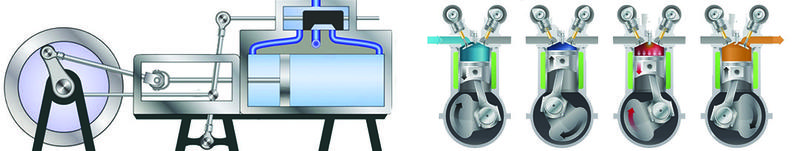
\includegraphics[width=12cm]{Images/dongco2}
\begin{center}
\textit{Động cơ hơi nước và động cơ đốt trong}
\end{center}
\end{center}
